%!TEX root = dissertacao.tex
\section{RESULTADOS}
\label{sec:resultadosParciais}
O presente projeto de pesquisa apresenta como resultado o desenvolvimento da operação de diferença entre templates com $k=2$, introduz a operação de templates de exceção e demonstra uma série de passos que, utilizando a operação de diferença, conseguem restringir o espaço busca de ACs de raio 3 que tem a possibilidade de solucionar o problema de paridade. E essa seção descreverá esses resultados encontrados.

\subsection{Templates de Exceção}
\textit{Templates de exceção} são um conjunto $C_e$ com $n$ templates em que cada um desses $n$ templates que apresentam um conjunto de substituições que levem o template passado com parâmetro $T_o$ a apresentar substituições fora do intervalo inteiro $[0, k-1]$. A operação que gera os templates de exceção pode ser descrita em mais detalhes da seguinte maneira:
\begin{equation}
\begin{split}
X(T_o)= C_e \\
C_e = \{T_1,T_2,\dots, T_n\}\\
\end{split}
\end{equation}

Para exemplificar essa operação, considere o template $T_o = (x_7, x_6, x_5, 1 - x_1 - x_2, 2 - x_1 - x_2, x_2, x_1, 0)$ para $k=2$. É trivial perceber que qualquer expansão do template $T_o$ que tenha o conjunto de substituições $\{x_1 = 1, x_2 = 1\}$ fará com que a posição 4 do template apresente o valor $2$, que não pertence ao intervalo $[0,k-1]$. Da mesma maneira, qualquer expansão do template $T_o$ que tenha o conjunto de substituições $\{x_1 = 0, x_2 = 0\}$ fará com que a posição 3 do template também apresente um valor que não pertence ao intervalo $[0,k-1]$. O que a operação geradora de templates de exceção faz é primeiramente encontrar todos os conjunto de substituições que levam o template passado como parâmetro a apresentar regra inválidas, que no caso de $T_o$ é o conjunto $R_{ex} = \{\{x_1 = 1, x_2 = 1\}, \{x_1 = 0, x_2 = 0\}\}$. Posteriormente, a operação geradora de templates aplica as substituições $R_{ex}$ ao template base, gerando assim o conjunto de templates $C_e$, que para o exemplo utilizado 
 pode ser representado pela Eq. \ref{eq:exceptionsTemplates}.
\begin{equation}
$C_e = \{(x_7, x_6, x_5, x_4, x_3, 1, 1, x_0),(x_7, x_6, x_5, x_4, x_3, 0, 0, x_0)\}$
\label{eq:exceptionsTemplates}
\end{equation}

A operação que gera os templates de exceção foi apresentada por Soares, Verardo e
de Oliveira (\citeyear{soares2016difference}) e é importante por ser essencial para a operação de diferença entre templates.

\subsection{Diferença entre Templates binários}
A operação de diferença entre templates binários é responsável por obter um conjunto $C_d$ com $n$ templates, onde esses templates quando expandidos apresentam apenas as regras geradas pela expansão do template $T_m$ que não estejam também presentes na expansão do template $T_s$. A operação de diferença pode ser descrita em mais detalhes da seguinte maneira:
\begin{equation}
\begin{split}
D(T_m,T_s)= C_d \Leftrightarrow E(C_d) = E(T_m) \setminus E(T_s) \\
C_d = \{T_1,T_2,\dots, T_n\}\\
\end{split}
\end{equation}

A Figura \ref{fig:complement} ilustra essa operação, onde os templates $T_m$ e $T_s$ passados como parâmetro para a operação de diferença estão representado pelos dois círculos, e o conjunto $C_d$ retornado pela função está representado pela área em cinza na imagem.
\begin{figure}[h!]
  \centering
  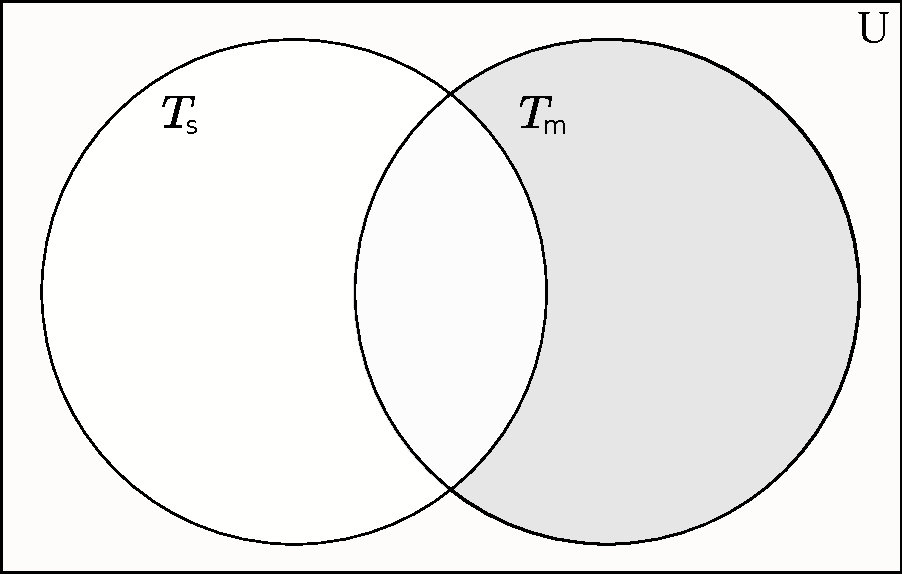
\includegraphics[width=.4\textwidth]{fig_complement2.pdf}
  \caption{Os círculos $T_m$ e $T_s$ são os templates que representam dois conjuntos de regras. Em cinza, $C_d$ é o conjunto de template que representa o conjunto de regras retornado pela operação de diferença entre $T_m$ e $T_s$.}
  \label{fig:complement}
\end{figure}    

O processo que o algoritmo usa para encontrar a diferença entre dois templates é efetuado através de uma sequência de etapas. A primeira etapa consiste em encontrar o template $T_i$, que é a intersecção entre os templates $T_m$ e $T_s$, ambos recebidos como parâmetro. Em seguida iguala-se os template $T_m$ e $T_i$ obtendo assim combinações lógicas de equações. Então o algoritmo remove as equações tautológicas, aplica uma operação de negação nas equações e troca o operador lógico $\wedge$ por $\vee$, no caso binário a operação de negação e a troca dos operadores consiste apenas em efetuar as permutações $\rho = (0 \rightarrow 1, 1 \rightarrow 0, \wedge \rightarrow \vee)$ ao resultado final das equações. Neste momento esse sistema é solucionado resultando num conjuntos com diversos conjuntos de regras de substituições que são aplicados ao template $T_i$, gerando assim um conjunto de templates que é parte do resultado dessa operação. Um segundo conjunto de templates será a outra parte do resultado. Esse conjunto será gerado apartir da intersecção de cada um dos templates de exceção do template $T_i$ com o template $T_m$.

Para melhor visualizar essas etapas, considere os template $T_m = (x_7, x_6, x_5, x_4, x_3, x_1, x_1, x_0)$ e $T_s = (x_7, x_6, x_3 + x_1, 1 - x_1, x_3, x_1, x_1, 0)$, ambos com $k=2$ e $r=1$. Esses templates serão primeiramente passados para a operação de intersecção, gerando assim o template $T_i = (x_7, x_6, x_3 + x_1, 1 - x_1, x_3, x_1, x_1, 0)$. Em sequencia, igualá-se os templates $T_m$ e $T_i$ gerando um sistema de equações representado pela Eq. \eqref{eq:complement}.
\begin{equation}
\left\{\begin{matrix}
x_7 & = & x_7	\\ 
x_6 & = & x_6	\\ 
x_5 & = & x_3 + x_1	\\ 
x_4 & = & 1 - x_1 \\ 
x_3 & = & x_3	\\ 
x_1 & = & x_1	\\ 
x_1 & = & x_1	\\ 
x_0 & = & 0
\end{matrix}\right.
\label{eq:complement}
\end{equation}

Esse sistema deve ser representado através de combinações lógicas de equações, como se pode ver na Eq. \eqref{eq:logicalComplement}, que é equivalente a Eq. \eqref{eq:complement}.
\begin{equation}
\begin{split}
x_7 = x_7	\wedge  
x_6 = x_6	\wedge  
x_5 = x_3 + x_1	\wedge  
x_4 =   1 - x_1 \wedge  \\
x_3 = x_3	\wedge  
x_1 = x_1	\wedge  
x_1 = x_1	\wedge  
x_0 = 0
\end{split}
\label{eq:logicalComplement}
\end{equation}

Antes de solucionar a Eq. \eqref{eq:logicalComplement}, o algoritmo elimina todas as equações tautológicas e troca todo operador lógico $\wedge$ por $\vee$. Ao se executar essas etapas na Eq. \eqref{eq:logicalComplement}, obtêm-se a Eq. \eqref{eq:logicalComplement1} ilustrada abaixo:
\begin{equation}
x_5 = x_3 + x_1 \vee x_4 = 1 - x_1 \vee x_0 = 0
\label{eq:logicalComplement1}
\end{equation}

Por fim é aplicado a operação de negação nas equações. No caso binário basta efetuar a permutação $\rho$, que também pode ser feita por meio da função $f(x) = 1 - (x)$. A Eq. \eqref{eq:logicalComplement2} representa a combinação lógica de equações resultante dessas operações.
\begin{equation}
x_5 = 1 - (x_3 + x_1) \vee x_4 = 1 - (1 - x_1) \vee x_0 = 1 - 0
\label{eq:logicalComplement2}
\end{equation}

Efetuado esses passos, a combinação lógica de equações resultante é solucionada obtendo-se o conjunto solução $S = \{\{x_0 \to 1\}, \{x_4 \to x_1\}, \{x_5 \to 1 - x_1 - x_3\}\}$. Perceba que $S$ apresenta mais de um conjunto de substituições, e cada um dos conjuntos de substituição deve ser utilizado para realizar as substituições no template $T_m$. Essas substituições faz com que se obtenha o conjunto de templates $C_{d1}$, representados pela Eq. \eqref{eq:logicalComplement3}. 
\begin{equation}
\begin{split}
C_{d1} = \{\\(x_7, x_6, x_5, x_4, x_3, x_1, x_1, 1), \\(x_7, x_6, x_5, x_1, x_3, x_1, x_1, x_0), \\(x_7, x_6, 1 - x_1 - x_3, x_4, x_3, x_1, x_1, x_0)\\\}
\end{split}
\label{eq:logicalComplement3}
\end{equation}

Os templates do conjunto $C_{d1}$ farão parte do conjunto $C_d$ resultante da operação de diferença. Entretanto é necessário verificar se o template $T_i$ possui combinações de substituições que o levem a gerar regras inválidas. Isso é feito passando o template $T_i$ para a operação geradora de template de exceção, obtendo-se o conjunto de templates ${(x_7, x_6, x_5, x_4, 1, x_2, 1, x_0)}$. Os templates desse conjunto são então interseccionados com o template $T_m$, resultando no conjunto $C_e = {(x_7, x_6, x_5, x_4, 1, 1, 1, x_0)}$. Por fim, se faz a unificação dos conjuntos $C_{d1}$ e $C_e$, finalizando a operação e obtendo-se o conjunto de templates $C_d$, representado pela Eq. \ref{eq:complementionSet}.
\begin{equation}
\begin{split}
C_{d1} = \{\\(x_7, x_6, x_5, x_4, x_3, x_1, x_1, 1), \\(x_7, x_6, x_5, x_1, x_3, x_1, x_1, x_0), \\(x_7, x_6, 1 - x_1 - x_3, x_4, x_3, x_1, x_1, x_0), \\(x_7, x_6, x_5, x_4, 1, 1, 1, x_0)\\\}
\label{eq:complementionSet}
\end{split}
\end{equation}

A implementação da operação de diferença foi desenvolvida na linguagem do software \textit{Wolfram Mathematica} \cite{woframMathematica10} e na mesma linguagem foi criado os testes unitários para essa operação. Todo testes receberam dois templates, $T_m$ e $T_s$, expandiram esses dois templates individualmente, e depois subtraíram das regras encontradas na expansão de $T_m$ todas as regras representadas por $T_s$. O resultado da diferença entre $T_m$ e $T_s$ é o conjunto de regras $C_{exp}$. Esse conjunto de regras $C_{exp}$ deve ser idêntico as regras geradas pela expansão dos templates resultantes da operação de diferença entre templates entre $T_m$ e $T_s$.

Obter a diferença entre regras representadas por dois templates por meio da expansão de ambos é uma operação muito custosa. Por conta disso os testes dessa operação se concentraram no raio 1, 2 e 3. Nos testes para todos os raios foi gerado um conjunto de templates, e a partir desse conjunto gerou-se todos os pares de combinações possíveis. Por fim, foi realizado o teste da operação de diferença com cada um dos pares de template gerados.

Para os testes com templates com $r = 1$, cada um dos templates do conjunto usado para o testes representava uma das seguintes propriedades estáticas: Conservabilidade de estados; confinamento; totalidade; semi-totalidade; e invariância a troca de cor. Além desse templates, também foi utilizado o template base, que representa todas as regras do espaço.

Para os testes com templates com $r = 2$, os templates do conjunto usado para o testes representavam as seguintes propriedades estáticas: Conservabilidade de estados; totalidade; semi-totalidade; invariância a troca de cor. Já para os testes com templates com $r = 3$, os templates de teste representavam apenas as propriedades estáticas de totalidade e semi-totalidade.

A realização desses testes permitiu o aprimoramento da operação de diferença ao evidenciar alguns erros de implementação no algoritmo, que foram prontamente corrigidos. Além disso, esses testes mostraram que a operação de diferença está funcionando para diversos templates, sem a necessidade de operações específicas para cadas uma deles.

É importante dizer que a implementação do algoritmo que executa a operação de diferença entre templates ainda não permite trabalhar com $k\neq 2$, pois a negação das equações são feitas por meio da função $f(x) = 1 - (x)$. Outra questão é que a operação de diferença poderia ser feita sem a necessidade de se fazer a intersecção entre os templates $T_m$ e $T_s$, mas ao utilizar a intersecção evita-se algumas etapas, assim como faz com que a operação tenha como resultado um número menor de templates.

\subsection{Aplicação da diferença entre Templates no problema de paridade}
O desenvolvimento da operação de diferença entre template permite diversas possibilidades de aplicação.
Uma possibilidade interessante é no problema de paridade. 
Ainda não se sabe se existem regras de raio 3 que solucionem o problema de paridade \cite{Betel2013}. 
Mas o uso de templates e suas operações podem ser uma forma interessante de restringir o conjunto de regras na busca dessa solução.

As regras dos ACs que solucionam o problema de paridade têm algumas propriedades estáticas que podem ser trivialmente percebidas. 
Um AC que resolva o problema de paridade sempre será contido, tendo em vista no problema de paridade as vizinhanças homogêneas não devem levar a transições de estado ativas, e está é a única restrição de variável dos templates contidos para AC binários. 
Vale frisar que o espaço das regras contidas de raio 3 ainda é um espaço muito grande, entretanto essa não é a única propriedade estática que um AC que resolva o problema de paridade contém. 
Para que um AC resolva problema de paridade também é necessário que ele não seja conservativo, visto que se a soma dos estados do AC não mudar, ele nunca convergirá como propõe o problema. 
Por fim, espera-se que um AC que resolva o problema de paridade seja conservativo de paridade.

Dado a possibilidade de se obter os templates para todas essas propriedades, é também possível utilizar as operações de diferença e intersecção para restringir o espaço de busca para a solução desse problema.
Para efetuar esta restrição, basta efetuar a intersecção do templates de confinamento com o template de conservabilidade de paridade, visto que ambas as propriedades são consideradas interessante. 
Posteriormente, deve-se efetuar a operação de diferença com o template obtido pela primeira intersecção com template das regras conservativas de estado, visto que essas regras conservativas de estado não podem resolver o problema de paridade.

Formalmente essas operações de conjuntos entre os templates pode ser representado através da Eq. \eqref{eq:operationsTemplateParidade}, sendo que $T_{confinado}$ representa o templates das regras confinadas, $T_{conservaparidade}$ representa o templates das regras que conservam a paridade e ${T}_{conservaestados}$ um template de regras conservativas. O resultado dessa operação é $T_{paridade}$, esse resultado representa um conjunto de templates que restringem um pouco mais as regras com possibilidades de solucionar o problema de paridade.
\begin{equation}
T_{paridade} = (T_{conservaparidade} \cap T_{confinado}) - {T}_{conservaestados}
\label{eq:operationsTemplateParidade}
\end{equation}